\documentclass[titlepage, a4paper]{article}
\usepackage[swedish]{babel}
\usepackage[utf8]{inputenc}
\usepackage{color}
\usepackage{graphicx}
\usepackage{etoolbox}
\usepackage{stringenc}
\usepackage{pdfescape}

% Sidformat
\usepackage{a4wide}

% Fixa Appendix-titlar
\usepackage[titletoc,title]{appendix}

% Bättre tabeller
\usepackage{tabularx}

% Bättre bildtexter
\usepackage[margin=10pt,font=small,labelfont=bf,labelsep=endash]{caption}

% Enkelt kommando som låter mig attgöra-markera text
\newcommand{\todo}[1] {\textbf{\textcolor{red}{#1}}}

% Nytt \paragraph låter oss ha onumrerade bitar
\makeatletter
\renewcommand\paragraph{\@startsection{paragraph}{4}{\z@}%
{-3.25ex\@plus -1ex \@minus -.2ex}%
{1.5ex \@plus .2ex}%
{\normalfont\normalsize\bfseries}}
\makeatother

%\providecommand{\LIPSlogga}{../mall/logga1.png}
\providecommand{\LIPSdatum}{\today}

%% Headers och Footers
\usepackage{fancyhdr}
\pagestyle{fancy}
%\lhead{\includegraphics[scale=0.4]{\LIPSlogga}}
\rhead{\ifdef{\LIPSutfardare}{Utfärdat av \LIPSutfardare \\\LIPSdatum}\LIPSdatum}
\lfoot{\LIPSkursnamn \\ \LIPSdokumenttyp}
\cfoot{\thepage}
\rfoot{\LIPSprojektgrupp \\ \LIPSprojektnamn}

%% Titelsida
\newcommand{\LIPSTitelsida}{%
{\ }\vspace{45mm}
\begin{center}
  \textbf{\Huge \LIPSdokument}
\end{center}
\begin{center}
  {\Large Redaktör: \LIPSredaktor}
\end{center}
\begin{center}
  {\Large \textbf{Version \LIPSversion}}
\end{center}
\vfill
\begin{center}
  {\large Status}\\[1.5ex]
  \begin{tabular}{|*{3}{p{40mm}|}}
    \hline
    Granskad & \LIPSgranskare & \LIPSgranskatdatum \\
    \hline
    Godkänd & \LIPSgodkannare & \LIPSgodkantdatum \\
    \hline
  \end{tabular}
\end{center}
\newpage
}

% Projektidentitet
\newenvironment{LIPSprojektidentitet}{%
{\ }\vspace{45mm}
\begin{center}
  {\Large PROJEKTIDENTITET}\\[0.5ex]
  {\small
  \LIPSartaltermin, \LIPSprojektgrupp\\
  Linköpings Tekniska Högskola, IDA
  }
\end{center}
\begin{center}
  {\normalsize Gruppdeltagare}\\
  \begin{tabular}{|l|l|p{25mm}|l|}
    \hline
    \textbf{Namn} & \textbf{Ansvar} & \textbf{Telefon} & \textbf{E-post} \\
    \hline
}%
{%
    \hline
  \end{tabular}
\end{center}
\begin{center}
  {\small
    \ifdef{\LIPSgruppadress}{\textbf{E-postlista för hela gruppen}: \LIPSgruppadress\\}{}
    \ifdef{\LIPSgrupphemsida}{\textbf{Hemsida}: \LIPSgrupphemsida\\[1ex]}{}
    \ifdef{\LIPSkund}{\textbf{Kund}: \LIPSkund\\}{}
    \ifdef{\LIPSkundkontakt}{\textbf{Kontaktperson hos kund}: \LIPSkundkontakt\\}{}
    \ifdef{\LIPSkursansvarig}{\textbf{Kursansvarig}: \LIPSkursansvarig\\}{}
    \ifdef{\LIPShandledare}{\textbf{Handledare}: \LIPShandledare\\}{}
  }
\end{center}
\newpage
}
\newcommand{\LIPSgruppmedlem}[4]{\hline {#1} & {#2} & {#3} & {#4} \\}

%% Dokumenthistorik
\newenvironment{LIPSdokumenthistorik}{%
\begin{center}
  Dokumenthistorik\\[1ex]
  %\begin{small}
    \begin{tabular}{|l|l|p{60mm}|l|l|}
      \hline
      \textbf{Version} & \textbf{Datum} & \textbf{Utförda förändringar} & \textbf{Utförda av} & \textbf{Granskad} \\
      }%
    {%
			\hline
    \end{tabular}
  %\end{small}
\end{center}
}

\newcommand{\LIPSversionsinfo}[5]{\hline {#1} & {#2} & {#3} & {#4} & {#5} \\}

% Kravlistor
\newenvironment{LIPSkravlista}{
	\center
		\tabularx{\textwidth}{| p{1.2cm} | p{1.9cm} | X | c |}
			\hline
			\textbf{Krav} & \textbf{Förändring} & \textbf{Beskrivning} & \textbf{Prioritet} \\\hline
}
{
		\endtabularx
	\endcenter
}

\newcounter{LIPSkravnummer}
\addtocounter{LIPSkravnummer}{1}
\newcommand{\LIPSkrav}[4][Krav \arabic{LIPSkravnummer}]{{#1} & {#2} & {#3} & {#4} \stepcounter{LIPSkravnummer}\\\hline}


% Leveranskravlistor
\newenvironment{LIPSleveranskravlista}{
	\center
		\tabularx{\textwidth}{| p{1.2cm} | p{1.9cm} | X | X |}
			\hline
			\textbf{Krav} & \textbf{Förändring} & \textbf{Beskrivning} & \textbf{Deadline}\\\hline
}
{
		\endtabularx
	\endcenter
}

\newcounter{LIPSleveranskravnummer}
\addtocounter{LIPSleveranskravnummer}{1}
\newcommand{\LIPSleveranskrav}[4][Krav \arabic{LIPSkravnummer}]{{#1} & {#2} & {#3} & {#4} \stepcounter{LIPSkravnummer}\\\hline}


% Milstolps-lista
\newenvironment{LIPSmilstolpar}{
	\center
		\tabularx{\textwidth}{| p{1.2cm} | X | l |}
			\hline
			\textbf{Nr} & \textbf{Beskrivning} & \textbf{Datum} \\\hline
}
{
		\endtabularx
	\endcenter
}

\newcounter{LIPSstolpnummer}
\addtocounter{LIPSstolpnummer}{1}
%\newcommand{\LIPSmilstolpe}[3][Krav \arabic{LIPSstolpnummer}]{{#1} & {#2} & {#3} \stepcounter{LIPSstolpnummer}\\\hline}
\newcommand{\LIPSmilstolpe}[3]{{#1} & {#2} & {#3} \\\hline}

% Aktivitets-lista
\newenvironment{LIPSaktivitetslista}{
	\center
		\tabularx{\textwidth}{| p{0.3cm} | X | c | c | c |}
			\hline
			\textbf{Nr} & \textbf{Beskrivning} & \textbf{Beroende av} & \textbf{Timmar} & \textbf{datum} \\\hline
}
{
		\endtabularx
	\endcenter
}

\newcounter{LIPSaktivitetsnummer}
\addtocounter{LIPSaktivitetsnummer}{1}
% \newcommand{\LIPSaktivitet}[4][\arabic{LIPSstolpnummer}]{{#1} & {#2} & {#3} & {#4} \stepcounter{LIPSstolpnummer}\\\hline}
\newcommand{\LIPSaktivitet}[5]{{#1} & {#2} & {#3} & {#4} & {#5}\\\hline}

% Mall för mötesprotokoll
\newenvironment{projektmote}[2]{
  {\ }\vspace{5mm}

  \centerline{\textbf{\Huge #1}}
  \vspace{2mm}
  \centerline{\LARGE #2}
  \vspace{10mm}

  \begin{itemize}
}
{
  \end{itemize}
}

\newcounter{paragrafnummer}
\addtocounter{paragrafnummer}{1}
\newcommand{\paragraf}[1]{\item{\textsection \arabic{paragrafnummer}. {#1}}\addtocounter{paragrafnummer}{1}}

% Mall för Statusrapport
\newenvironment{statusrapport}{
  \center
    \tabularx{\textwidth}{| p{0.4cm} | X | X | p{14.5mm} | p{13.5mm} | p{16.5mm} | p{16.5mm} |}
    \hline
    \textbf{Nr} & \textbf{Aktivitet} & \textbf{Beroenden} & \textbf{Planerad tid} & \textbf{Nedlagd tid} & \textbf{Planerad klar} & \textbf{Beräknat klart} \\\hline
}
{
    \endtabularx
  \endcenter
}

\newcommand{\aktivitetstatus}[7]{{#1} & {#2} & {#3} & {#4} & {#5} & {#6} & {#7} \\\hline}	% Importera generella layout-strukturer

% Information nödvändig för generella layout-strukturer
\newcommand{\LIPSredaktor}{Johannes Klasson}
\newcommand{\LIPSversion}{0.1}
\newcommand{\LIPSdokument}{Projektplan}
	\newcommand{\LIPSdokumenttyp}{Projektplan}
\newcommand{\LIPSgranskatdatum}{-}
\newcommand{\LIPSgranskare}{Johannes Klasson}
\newcommand{\LIPSgodkannare}{Martin Nielsen Lönn}
\newcommand{\LIPSgodkantdatum}{-}
\newcommand{\LIPSkursnamn}{TSEK06}
\newcommand{\LIPSprojektnamn}{16-bit Adder}
\newcommand{\LIPSprojektgrupp}{Grupp 5}
%\newcommand{\LIPSgruppadress}{\todo{Ta bort}}
\newcommand{\LIPSartaltermin}{VT, 2016}
\newcommand{\LIPSgrupphemsida}{-}
\newcommand{\LIPSkund}{ISY}
\newcommand{\LIPSkundkontakt}{Martin Nielsen Lönn}
\newcommand{\LIPSkursansvarig}{Atila Alvandpour}
\newcommand{\LIPShandledare}{Martin Nielsen Lönn}

% Dokument-specifika paket
\usepackage{tabularx}
\usepackage{pdfpages}
\usepackage{tikz}
\usepackage{float}
\usetikzlibrary{shapes, arrows}

\pagenumbering{roman}


\DeclareGraphicsRule{.0.pdf}{pdf}{*}{}

\begin{document}

\LIPSTitelsida

\begin{LIPSprojektidentitet}
	\LIPSgruppmedlem{Johan Isaksson}{Projektledare}{070 2688785}{johis024@student.liu.se}
	\LIPSgruppmedlem{Johannes Klasson}{Dokumentansvarig}{073 8209003}{johkl226@student.liu.se}
	\LIPSgruppmedlem{Jonas Tarasso}{Designer}{070 5738583}{jonta760@student.liu.se}
	\LIPSgruppmedlem{Alexander Yngve}{Designer}{076 2749762}{aleyn573@student.liu.se}	
\end{LIPSprojektidentitet}

\newpage
\tableofcontents	%Innehållsförteckning
%\listoffigures
%\listoftables

\newpage

\begin{LIPSdokumenthistorik}
\LIPSversionsinfo{0.1}{2016-02-10}{Första utkast}{Johan Isaksson}{}
\end{LIPSdokumenthistorik}

\newpage
\pagenumbering{arabic}	%Påbörja sidnumrering

% Inledning, översikt osv

\section{Beställare}

Beställare är SAAB med Daniel Simon som kontaktperson.

\section{Översiktlig beskrivning av projektet}


\subsection{Syfte och mål}
Syftet med projektet är att:
\begin{enumerate}
 \item Gruppen systematiskt ska integrera sina kunskaper som har förvärvats under studietiden, främst inom programmering och datalogi. 
 \item Tillämpa sig  metodkunskaper och ämnesmässiga kunskaper inom datateknik.
 \item Tillgodogöra sig innehållet i relevant facklitteratur och relatera sitt arbete till den.
\end{enumerate}

\raggedright Målet med projektet är att välja ut en lämplig algoritm som löser kvadratiska optimeringsproblem och sedan implementera den effektivt. Denna implementation ska sedan användas för att lösa prediktionsregleringsproblem åt SAAB. 

\subsection{Leveranser}

%H fungerar inte utan float paketet
\begin{table}[H]
  \centering
    \begin{tabularx}{\textwidth}{| X | l | X | X |}
      \hline
      \textbf{Leverans} & \textbf{Ansvarig} & \textbf{Beskrivning} & \textbf{Färdig} \\
      \hline

      {Projekt och teamledare} & {Adam Sestorp} & {Projektval och val av teamledare ska vara inlämnat till examinator} & {2015-01-23} \\
            \hline
      {Avtal} & {Adam Sestorp} & {Kopia på avtal med kunden ska vara påskrivet och inlämnat till examinatorn} & {2015-02-03} \\
      \hline
      {Förstudiedokument} & {Adam Sestorp} & {Kravspecifikation och projektplan ska vara inlämnade till handledare och opponentgrupp} & {2015-02-16} \\
      \hline
      {Förstudiedokument} & {Ruben Das} & {Kvalitetsplan ska vara inlämnad till handledare och eventuellt kund} & {2015-02-16} \\
      \hline
      {Förstudiedokument} & {Sebastian Fast} & {Första utkast av arkitektplan ska vara påbörjat} & {2015-02-16} \\
      \hline
      {Förstudiedokument} & {Johan Isaksson} & {Första utkast av testplan ska vara påbörjat} & {2015-02-16} \\
      \hline
      {Dokument} & {Adam Sestorp} & {Inlämning av halvtids-dokument till handledare och opponentgrupp} & {2015-03-13} \\
      \hline
      {Rapport} & {Adam Sestorp} & {Utkast 1 av slutrapporten ska vara inlämnat till handledare och opponentgrupp} & {2015-03-13} \\
      \hline
      {Dokument} & {Adam Sestorp} & {Dokument för iteration 2 ska vara inlämnade till handledaren} & {2015-04-20} \\
      \hline
      {Rapport} & {Adam Sestorp} & {Utkast 2 av slutrapporten ska vara inlämnade till handledare opponentgrupp och examinator} & {2015-05-13} \\
      \hline
      {Rapport} & {Adam Sestorp} & {Slutrapport ska vara färdig och inlämnad till handledare och examinator} & {2015-05-27} \\
      \hline
      {Statusrapport} & {Adam Sestorp} & {Statusrapport ska lämnas in till berörda} & {Varje vecka till handledaren. Vid begäran till kund.} \\
      \hline
      {Delleverans} & {Martin Söderén} & {Det som har producerats skickas till kunden} & {Vid sluten av varje iteration} \\
      \hline

    \end{tabularx}
  \caption{Projektets leveranser.} \label{dokumentation:tabell}
\end{table}



\subsection{Begränsningar}

Projektet är begränsat till att uppfylla de krav som angetts i kravspecifikationen. De krav i kravspecifikationen som angetts med annan prioritet än 1 kommer endast att genomföras i mån av tid. Det finns även begränsningar på hur många timmar som kan läggas på projektet. Från det att förstudien inleds så får varje gruppmedlem max spendera 300 timmar på projeketet. Utöver detta får det max skilja 10\% mellan medlemmer i nedlagd tid.

\section{Fasplan}
Projektet består av fem faser och Alfa-tillstånden finns med i bilaga B:
\begin{enumerate}
\item Förstudie
\item Iteration 1
\item Iteration 2
\item Iteration 3
\item Redovisning och reservtid
\end{enumerate}

\subsection{Förstudie}
Innan iteration 1 genomförs en förstudie där en  kravspecifikation, en projektplan och en kvalitetsplan ska skrivas och lämnas in till handledaren samt kund. 

\subsection{Under iterationerna}

Under projektets gång skall handledaren kontinuerligt uppdateras hur projektet fortskrider genom tidsrapporter varje vecka. I slutet av varje iteration ska diverse dokument lämnas in för att ge intressenter en insikt i hur arbetet fortskrider. Även en statusrapport ska kunna skickas iväg till handledaren varje vecka eller kund om det begärs. 


\subsection{Efter projektet}
Efter iteration 3 ska resultatet granskas vid en opponering där projektet både blir granskat och där gruppen opponerar mot ett annat projekt. Sedan följer en inlämning av en slutrapport, en demonstration av resultatet och överlämning till beställaren. 


\section{Organisationsplan för hela projektet}
Beställning av projektet har gjorts av kunden, och det är kunden som levererat kravspecifikationen och på så sätt avgör om den är uppfylld eller inte. Det är även kunden som står för betalning av den slutgiltliga produkten, som i detta fall kommer vara i form av högskolepoäng. All kontakt med kunden och annan kontakt utåt ligger på projektledaren. Projektledaren ska också planera arbetet i gruppen och se till att hela gruppen arbetar mot ett och samma mål. Arbetet i sig ligger dock inte enbart på projektledarens axlar, utan även på resterande gruppmedlemmar, där alla, inklusive projektledaren, spelar lika stor roll i arbetets utförande. Det finns även en handledare tillgänglig som experthjälp för att hjälpa gruppen på vägen. Figur \ref{organisationsplan} illustrerar organisationsstrukturen.

\begin{figure}[H]
	\begin{center}
		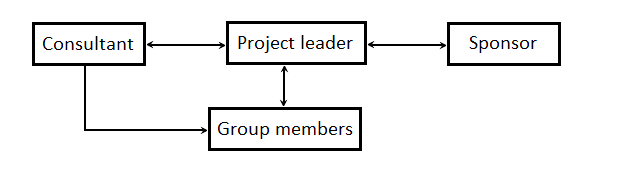
\includegraphics[keepaspectratio=true,width=375px]{grafik/organisationsplan.png}
		\caption{Organisationsplan}
		\label{organisationsplan}
	\end{center}
\end{figure}

\subsection{Villkor för samarbete inom projektgruppen}
Inom gruppen har vi kommit överens om att följande gäller:
\begin{itemize}
\item{Alla skall komma väl förberedda till möten.}
\item{Meddela i tid om man inte kan närvara vid ett möte. Vid sjukdom skall detta meddelas snarast.}
\item{Man skall delta vid möten som gruppen kommit överens om.}

\item{Om man är osäker på något ska man först söka information på egen hand eller ta upp detta med gruppen. I andra hand bör någon extern person tas kontakt med.}
\item{Om någon inte bidrar tillräckligt till projektet så har resterande gruppmedlemmar rätt att diskutera detta med handledare.}
\end{itemize}

\newpage

\section{Documentation}
The documentation listed in table \ref{dokumentation:tabell} shall be delivered to the sponsor.

\begin{table}[H]
	\centering
		\begin{tabularx}{\textwidth}{| l | X | l |}
			\hline
			\textbf{Dokument} & \textbf{Syfte} & \textbf{Färdig datum} \\\hline
			
			{Project plan} & {This is an aid for the project group, describing some basics needed for the collaboration of the project group. This will also include a time plan.} & {2016-01-31} \\\hline
			
			{High-level design report} & {It should include the complete block level description of the project. Simulation results that verifies the desired functionality should be included. An updated time plan and a time report should be included as well.} & {2016-02-19} \\\hline
			
			{Transistor design report} & {It should include the complete block level description of the project. Simulation results that verifies the desired functionality should also be included. An updated time plan a, a time report, PAD assignments and an early test plan should be included as well. } & {2016-03-18} \\\hline
			
			{Final report} & {Block level from the two previous reports should be included along with simulation results of the final design. A final time report, an evaluation plan and a PAD list should also be included. A short evaluation of the projecy should be included as well.} & {2016-05-27} \\\hline
			
			
		\end{tabularx}
	\caption{Dokumentation.} \label{dokumentation:tabell}
\end{table}


% \section{Utvecklingsmetodik}

\todo{Skiter i't}

%\section{Utbildningsplan}
En del utbildning kommer behövas för att samtliga gruppmedlemmar ska förstå problemet som ska lösas samt lära sig de nödvändiga färdigheterna. 

\subsection{Egen utbildning}
Gruppen ska ha en gemensam utbildning i konvexa kvadratiska optimeringsproblem och lösningsmetoder för dessa. Standarderna för kod och versionshantering som gruppen valt att följa ska gås igenom med hela gruppen gemensamt. Utbildning i olika mjukvaror kommer även behövas. Se utbildningsaktiviteter i 11.1. 

\subsection{Övrig utbildning}
All utbildning som krävs för projektet har införskaffats under studieperioden här på Linköpings universitet samt på fritid. Därför behövs ingen övrig utbildning.

\section{Rapporteringsplan}
Rapporter kommer att användas för att ge beställaren, handledaren och examinatorn en bild av hur projektet fortlöper och om tiden fördelas efter anvisningar. Projekledaren är ansvarig för att dessa rapporter skrivs och levereras enligt överenskommelse.

\subsection{Statusrapport}
Varje vecka skall en statusrapport levereras till handledaren. Statusrapporten ska innehålla vad som har gjorts och hur mycket tid som har lagts ner sedan den senaste statusrapporten, samt vilka problem som kommit upp.



%\section{Mötesplan}

Regelbundna möten ska hållas minst en gång i veckan, närmare bestämt på måndagar vid en tid som gruppen gemensamt bestämmer i god tid innan mötet ska genomföras. Mötets agenda går ut på att stämma av vart vi befinner oss i projektet, eventuella problem som har uppkommit samt vad som ska göras härnäst. Varje gruppmedlem ska kunna redogöra för sin genomförda, pågående och kommande aktiviteter samt besvara frågor rörande detta. En mall för möten finns i bilaga A.


\section{Resursplan}

\subsection{Personer}
Projektgruppen består av medlemmar enligt tabell \ref{projektplan:resursplan-personer}
\begin{table}[h]
	\centering
		\begin{tabularx}{\textwidth}{| l | l | X | l | l | l |}
			\hline
			\textbf{Namn} & \textbf{Ansvar} & \textbf{E-post} \\
			\hline
			{Adam Sestorp} & {Teamleader} & {adase035@student.liu.se} \\\hline
			{Dennis Ljung} & {Dokumentansvarig} & {denlj069@student.liu.se} \\\hline
			{Alexander Yngve} & {Utvecklingsansvarig} & {aleyn573@student.liu.se} \\\hline
			{Martin Söderén} & {Analysansvarig} & {marso329@student.liu.se} \\\hline
			{Ruben Das} & {Kvalitetssamordnare} & {rubdas680@student.liu.se} \\\hline
			{Sebastian Fast} & {Arkitekt} & {sebfa680@student.liu.se} \\\hline
			{Johan Isaksson } & {Testledare} & {johis024	@student.liu.se} \\\hline
		\end{tabularx}
	\caption{Medlemmar i projektgruppen} \label{projektplan:resursplan-personer}
\end{table}

\subsection{Material}
Material nödvändig för projektet kommer dels att förses av beställaren, dels av oss själva. Testdata så programmet kan testas kommer förses av beställaren och mjukvarorna Matlab och Gurobi kommer vi i gruppen behöva införskaffa själva. Matlab är gratis för studenter och Gurobi finns gratis som trial-version.  

\subsection{Lokaler}
Vi har inte tillgång till några lokaler. Arbete och alla möten sker i skolans lokaler som vi bokar dagen innan. 

\subsection{Ekonomi}
Varje medlem i projektet har 300 timmar att lägga på projektet. Detta betyder att projektetet när det är klart ska ha förbrukat 2100 minus eventuell variation mellan gruppmedlemmarna som maximalt för överstiga tio procent. Eventuell buffertid ska disponeras på aktiviteter som dragit över tiden. 

\section{Milstolpar och beslutspunkter}
Milstolpar är organiserade så att grundläggande funktioner implementeras först. En milstolpe anses vara avklarad när funktionaliteten är väl testad och de underliggande funktionerna är väl dokumenterade.

\subsection{Milstolpar}
Nedan följer milstolpar uppsatta för projektet.
\begin{LIPSmilstolpar}

\LIPSmilstolpe{1}{Förstudie klar}{2015-02-16}
\LIPSmilstolpe{2}{Programmet ska ha grundläggande funktionalitet}{Iteration 1}
\LIPSmilstolpe{3}{Gränsnitt mellan systemets moduler klar}{Iteration 1}
\LIPSmilstolpe{4}{Algoritmen kan lösa ett konvext problem}{Iteration 1}
\LIPSmilstolpe{5}{Gränsnitt till Matlab klart}{Iteration 2}
\LIPSmilstolpe{6}{Parsern klar}{Iteration 2}
\LIPSmilstolpe{7}{GUI:t klart}{Iteration 3}
\LIPSmilstolpe{8}{QuadOpts prestanda är någorlunda likvärdig med prestandan hos Gurobi}{Iteration 3}
\LIPSmilstolpe{9}{Demonstration godkänd}{2015-05-27}
\end{LIPSmilstolpar}

\newpage

\section{Activities}
This chapter describes activities and tasks needed for each of the modules/subsystems in this project.

\subsection{SPI}
The following activities should be carried out to implement the Serial Peripheral unit.
\begin{LIPSaktivitetslista}
	\LIPSaktivitet{1}{Define structure of the SPI unit}{}{10}{phase 2}	
	\LIPSaktivitet{2}{Implement counters in Verilog-A}{1}{10}{phase 2}
	\LIPSaktivitet{3}{Implement control logic in Verilog-A}{1}{10}{phase 2}
	\LIPSaktivitet{4}{Implement 1:4 decoder in Verilog-A}{1}{10}{phase 2}
	\LIPSaktivitet{5}{Integrate to high level design of SPI}{2,3,4}{10}{phase 2}
	\LIPSaktivitet{44}{Implementation of test bench for SPI}{5}{5}{phase 2}
	\LIPSaktivitet{6}{Simulation and test of high level design}{5}{5}{phase 2}
	\LIPSaktivitet{7}{Implement transistor level design of the SPI unit}{5}{30}{phase 3}
	\LIPSaktivitet{8}{Simulation and test of transistor design}{7}{20}{phase 3}
	\LIPSaktivitet{9}{Implement layout level design of SPI unit}{8}{30}{phase 4}
	\LIPSaktivitet{10}{Simulation and test of layout}{9}{20}{phase 4}
\end{LIPSaktivitetslista}

\subsection{Number generator}
The following activities should be carried out to implement a number generator using pseudo random bit sequence (PRBS).
\begin{LIPSaktivitetslista}
	\LIPSaktivitet{11}{Define structure the generator}{}{10}{phase 2}
	\LIPSaktivitet{12}{Implement linear feedback shift registers in Verilog-A}{11}{10}{phase 2}
	\LIPSaktivitet{13}{Integrate to high level design of the generator}{12}{10}{phase 2}
	\LIPSaktivitet{45}{Implementation of test bench for generator}{13}{5}{phase 2}
	\LIPSaktivitet{14}{Simulation and test of the high level design}{13}{5}{phase 2}
	\LIPSaktivitet{15}{Implement transistor level design of the generator}{14}{15}{phase 3}
	\LIPSaktivitet{16}{Simulation and test of the transistor}{15}{10}{phase 3}
	\LIPSaktivitet{17}{Implement layout level design of generator unit}{16}{15}{phase 4}
	\LIPSaktivitet{18}{Simulation and test of layout}{17}{10}{phase 4}
\end{LIPSaktivitetslista}

\newpage
\subsection{Kogge-Stone adder}
The following activities should be carried out to implement the adder.
\begin{LIPSaktivitetslista}
	\LIPSaktivitet{19}{Define structure of the adder}{}{10}{phase 2}
	\LIPSaktivitet{20}{Implement Generate calculation logic in Verilog-A}{19}{10}{phase 2}
	\LIPSaktivitet{21}{Implement Propagate calculation logic in Verilog-A}{19}{10}{phase 2}
	\LIPSaktivitet{22}{Implement Sum calculation logic in Verilog-A}{19}{10}{phase 2}		
	\LIPSaktivitet{23}{Integrate to high level design of the adder}{20,21,22}{20}{phase 2}
	\LIPSaktivitet{46}{Implementation of test bench for the adder}{23}{10}{phase 2}
	\LIPSaktivitet{24}{Simulation and test of the high level design}{23}{10}{phase 2}
	\LIPSaktivitet{25}{Implement transistor level design of the adder}{24}{40}{phase 3}
	\LIPSaktivitet{26}{Simulation and test of the transistor design}{25}{20}{phase 3}
	\LIPSaktivitet{27}{Implement layout level design of adder unit}{26}{40}{phase 4}
	\LIPSaktivitet{28}{Simulation and test of layout}{27}{20}{phase 4}
\end{LIPSaktivitetslista}

\subsection{Comparator}
The following activities should be carried out to implement the the output comparator.
\begin{LIPSaktivitetslista}
	\LIPSaktivitet{29}{Define the structure of the comparator}{}{5}{phase 2}
	\LIPSaktivitet{30}{Implement bit comparator in Verilog-A}{29}{5}{phase 2}
	\LIPSaktivitet{31}{Integrate to high level design of the comparator}{30}{10}{phase 2}
	\LIPSaktivitet{47}{Implementation of test bench for the comparator}{30}{5}{phase 2}
	\LIPSaktivitet{32}{Simulation and test of the high level design}{31}{5}{phase 2}
	\LIPSaktivitet{33}{Implement transistor level design of the comparator}{32}{10}{phase 3}
	\LIPSaktivitet{34}{Simulation and test of the transistor design}{33}{20}{phase 3}
	\LIPSaktivitet{35}{Implement layout level design of adder unit}{34}{10}{phase 4}
	\LIPSaktivitet{36}{Simulation and test of layout}{35}{10}{phase 4}
\end{LIPSaktivitetslista}

\subsection{System integration}
The following activities should be carried out to integrate the modules together.
\begin{LIPSaktivitetslista}
	\LIPSaktivitet{41}{High level integration}{5,13,23,31}{15}{phase 2}
	\LIPSaktivitet{48}{Implementation of test bench for the complete system}{37}{20}{phase 2}
	\LIPSaktivitet{42}{Transistor level integration}{5,13,23,31}{10}{phase 3}
	\LIPSaktivitet{43}{Layout level integration}{5,13,23,31}{15}{phase 4}
\end{LIPSaktivitetslista}

\subsection{Chip assembly}
The following activity should be carried out to be able to manufacture the chip.
\begin{LIPSaktivitetslista}
	\LIPSaktivitet{37}{Off-chip hardware interface}{10,18,27,36}{20}{phase 5}
\end{LIPSaktivitetslista}

\subsection{Documentation}
The following activity should be carried out to provide satisfactory documentation.
\begin{LIPSaktivitetslista}
	\LIPSaktivitet{38}{Documentation and presentation}{}{60}{phase 2,3,4,5}
\end{LIPSaktivitetslista}

\subsection{Planning}
The following activities should be carried out for administrative work.
\begin{LIPSaktivitetslista}
\LIPSaktivitet{39}{Meetings}{}{60}{phase 2,3,4,5}
\LIPSaktivitet{40}{Buffer time}{}{80}{phase 2,3,4,5}
\end{LIPSaktivitetslista}




%\input{tex/projektplan-tidplan}

%\section{Förändringsplan}

I första hand skall förseningar hanteras internt i gruppen genom att justera tidsplanen. Om en försening är så stor att den riskerar att försena en leverans skall projektledaren ta kontakt med beställaren för att diskutera möjliga lösningar. Omförhandlingar av kravspecifikation och leveransdatum skall undvikas.

%\input{tex/projektplan-kvalitetsplan}

% \section{Prioriteringar}

\section{Projektavslut}

Projektet avslutas när produkten är acceptanstestad, levererad och både teknisk dokumentation och användarhandledning blivit levererade. 

%\section{Referenser}

\newpage
\begin{appendices}
	\section{Mötesmall} \label{ap:motesmall}
	\vspace{10mm}

\begin{itemize}
\item{\textsection 1. Mötet öppnas av teamledare alternativt tillförordnad teamledare.}
\item{\textsection 2. Sekreterare utses. Normalt utses dokumentansvarig.}
\item{\textsection 3. Varje gruppmedlem får några minuter att redogöra för sitt arbetes status.
  \begin{itemize}
  \item{Hur går arbetet?}
  \item{Medlemmen får uppskatta om denne tror att veckans aktiviteter kommer att hinnas med. Behövs ytterligare timmar eller eventuellt en till gruppmedlem tilldelas aktiviteten?}
  \item{Är medlemmen sjuk och arbetsuppgiften ligger som beroende hos andra aktiviteter, måste uppgiften isåfall överlämnas till en annan gruppmedlem?}
  \item{Är medlemmen redan klar med veckans aktiviteter?}
  \end{itemize}
}

\item{\textsection 4. Diskussion om eventuella problem i \textsection 3.
  \begin{itemize}
  \item{Ska samliga medlemmar närvara för att diskutera problemen?}
  \end{itemize}
}

\item{\textsection 5. Mötet avslutas.}
\end{itemize}



\end{appendices}

\end{document}
